\documentclass[border=8pt]{standalone}
\usepackage[T1]{fontenc}
\usepackage{mathptmx}
\usepackage{tikz}
\usetikzlibrary{arrows.meta,positioning,fit,calc,shapes.geometric,shapes.misc,shapes.multipart,backgrounds}
\tikzset{
  arr/.style={-{Stealth[length=2.4mm,width=1.8mm]},line width=0.6pt},
  box/.style={draw,line width=0.6pt,align=center,rounded corners=2pt},
}

\begin{document}
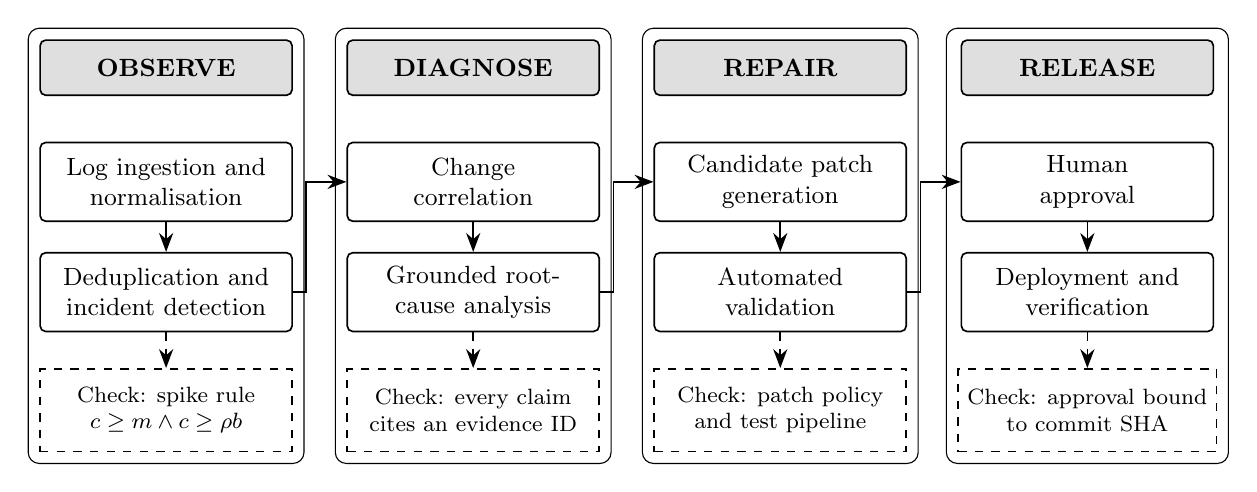
\begin{tikzpicture}[font=\small, s/.style={box, minimum width=3.2cm, minimum height=1.0cm}, h/.style={box, fill=gray!25, minimum width=3.2cm, minimum height=0.7cm, font=\small\bfseries}, c/.style={draw, dashed, line width=0.6pt, minimum width=3.2cm, minimum height=1.05cm, align=center, font=\footnotesize}]
\foreach \x/\p/\a/\b/\k [count=\i] in {
 0/OBSERVE/{Log ingestion and\\ normalisation}/{Deduplication and\\ incident detection}/{Check: spike rule\\ $c \geq m \wedge c \geq \rho b$},
 3.9/DIAGNOSE/{Change\\ correlation}/{Grounded root-\\cause analysis}/{Check: every claim\\ cites an evidence ID},
 7.8/REPAIR/{Candidate patch\\ generation}/{Automated\\ validation}/{Check: patch policy\\ and test pipeline},
 11.7/RELEASE/{Human\\ approval}/{Deployment and\\ verification}/{Check: approval bound\\ to commit SHA}}{
 \node[h] (h\i) at (\x,0) {\p};
 \node[s] (a\i) at (\x,-1.45) {\a};
 \node[s] (b\i) at (\x,-2.85) {\b};
 \node[c] (k\i) at (\x,-4.35) {\k};
 \draw[arr] (a\i)--(b\i); \draw[arr,dashed] (b\i)--(k\i);
 \begin{scope}[on background layer]\node[draw, line width=0.4pt, rounded corners=4pt, fit=(h\i)(k\i), inner sep=4pt] {};\end{scope}
}
\foreach \i [evaluate=\i as \j using int(\i+1)] in {1,2,3}{\draw[arr] (b\i.east) -- ++(0.17,0) |- (a\j.west);}
\end{tikzpicture}
\end{document}
